% ExternE impact-pathway approach.
% Compile to SVG:  latex impact_pathway.tex && dvisvgm --no-fonts impact_pathway.dvi -o ../impact_pathway.svg
\documentclass[tikz,border=6pt]{standalone}
\usepackage[scaled]{helvet}
\renewcommand{\familydefault}{\sfdefault}
\usetikzlibrary{arrows.meta,positioning}
\definecolor{blu}{HTML}{3B6EA8}
\definecolor{accent}{HTML}{2E7D32}
\begin{document}
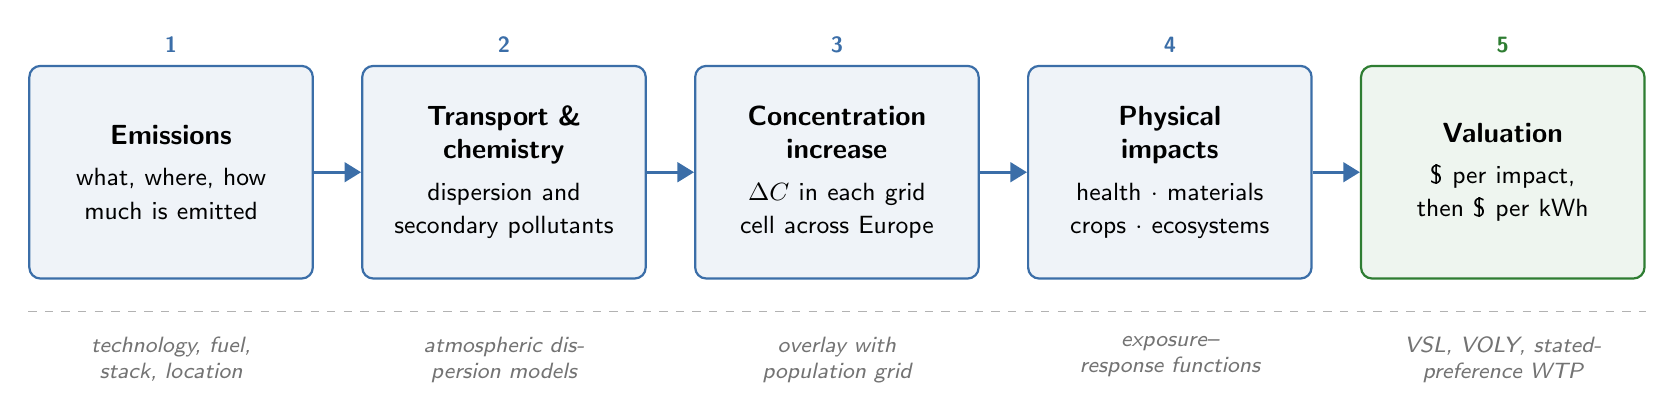
\begin{tikzpicture}[
    stage/.style={draw=blu, fill=blu!8, thick, rounded corners=4pt,
                  minimum width=3.6cm, minimum height=2.7cm, align=center,
                  text width=3.3cm},
    final/.style={stage, draw=accent, fill=accent!8},
    flow/.style={-{Triangle[length=6pt]}, very thick, blu},
    input/.style={font=\footnotesize\itshape, text=black!55, align=center, text width=3.4cm},
    num/.style={font=\footnotesize\bfseries, text=blu}]
  \node[stage] (e) {\textbf{Emissions}\\[3pt]\small what, where, how much is emitted};
  \node[stage, right=0.6cm of e] (t) {\textbf{Transport \&\\chemistry}\\[3pt]\small dispersion and secondary pollutants};
  \node[stage, right=0.6cm of t] (c) {\textbf{Concentration\\increase}\\[3pt]\small $\Delta C$ in each grid cell across Europe};
  \node[stage, right=0.6cm of c] (i) {\textbf{Physical\\impacts}\\[3pt]\small health $\cdot$ materials crops $\cdot$ ecosystems};
  \node[final, right=0.6cm of i] (v) {\textbf{Valuation}\\[3pt]\small \$ per impact, then \$ per kWh};
  \foreach \a/\b in {e/t, t/c, c/i, i/v} \draw[flow] (\a) -- (\b);
  \foreach \n/\k in {e/1, t/2, c/3, i/4} \node[num, above=1pt of \n] {\k};
  \node[num, text=accent, above=1pt of v] {5};
  \draw[black!30, dashed] ([yshift=-0.4cm]e.south west) -- ([yshift=-0.4cm]v.south east);
  \node[input, below=0.6cm of e] {technology, fuel, stack, location};
  \node[input, below=0.6cm of t] {atmospheric dispersion models};
  \node[input, below=0.6cm of c] {overlay with population grid};
  \node[input, below=0.6cm of i] {exposure--response functions};
  \node[input, below=0.6cm of v] {VSL, VOLY, stated-preference WTP};
\end{tikzpicture}
\end{document}
